% Shared preamble for the three ENS003 software-team presentations.
% Each presentation \input{}'s this file.

\documentclass[11pt,aspectratio=169]{beamer}

\usepackage[utf8]{inputenc}
\usepackage[T1]{fontenc}
\usepackage{lmodern}
\usepackage{amsmath}
\usepackage{booktabs}
\usepackage{graphicx}
\usepackage{listings}
\usepackage{xcolor}
\usepackage{hyperref}

% Built-in Beamer theme so the deck compiles on any TeX Live / MacTeX
% install without external packages. Customise colours below.
\usetheme{Boadilla}
\usecolortheme{seahorse}
\setbeamertemplate{navigation symbols}{}
\setbeamertemplate{footline}[frame number]

\definecolor{ink}{HTML}{1A1A1A}
\definecolor{accentred}{HTML}{A02828}
\definecolor{accentgreen}{HTML}{2C662C}
\definecolor{codebg}{HTML}{F7F5EE}
\definecolor{rulegrey}{HTML}{888888}

\setbeamercolor{normal text}{fg=ink}
\setbeamercolor{frametitle}{bg=ink, fg=white}
\setbeamercolor{title}{fg=ink}
\setbeamercolor{author}{fg=ink}
\setbeamercolor{date}{fg=rulegrey}
\setbeamercolor{block title}{bg=ink, fg=white}
\setbeamercolor{block body}{bg=codebg, fg=ink}
\setbeamercolor{alerted text}{fg=accentred}
\setbeamercolor{structure}{fg=ink}
\setbeamerfont{frametitle}{series=\bfseries}

\lstset{
  basicstyle=\ttfamily\scriptsize,
  backgroundcolor=\color{codebg},
  language=Python,
  keywordstyle=\color{accentred},
  stringstyle=\color{accentgreen},
  commentstyle=\color{rulegrey}\itshape,
  breaklines=true,
  numbers=none,
  showstringspaces=false,
  frame=single,
  framerule=0pt,
  framesep=6pt,
  xleftmargin=0pt,
  xrightmargin=0pt
}

% Convenience commands
\newcommand{\code}[1]{\texttt{\small #1}}
\newcommand{\file}[1]{\textcolor{accentred}{\texttt{\small #1}}}
\newcommand{\unit}[1]{\,\mathrm{#1}}

% Title-slide metadata is set per-deck (so the same preamble can power
% both Turkish and English versions of each talk).


\newcommand{\courseHeader}{ENS003 --- Digital Twins for Health Sciences}
\newcommand{\courseSubheader}{İstinye Üniversitesi · Müh. ve Doğa Bilimleri Fakültesi}
\newcommand{\instructor}{Eğitmen: Prof. Dr. Şenol Pişkin}
\newcommand{\projectTitle}{Ti-6Al-4V Çimentosuz Kalça İmplantı için Surrogate ML Modeli}

\title{Flask Dashboard, Predict CLI ve Entegrasyon}
\subtitle{\projectTitle}
\author{Ali Edip Mangtay \\ \small Yazılım Mühendisliği · 210911044}
\date{Mayıs 2026 \\ \scriptsize \courseHeader{} · \instructor}

\begin{document}

\maketitle

% ---------------------------------------------------------------------------
\begin{frame}{Bu sunumda}
  \begin{itemize}
    \item Surrogate'i son kullanıcının önüne taşıma görevi
    \item Mimari seçimleri (Flask + Jinja + Plotly + KaTeX)
    \item LaTeX-paper estetiği ve neden bu yola gidildi
    \item Sidebar UX: üç sürekli slider + üç preset butonu
    \item Production'a bakan bug'ları (500 hatası, cache)
  \end{itemize}
  \vspace{0.4cm}
  \begin{block}{Sorumluluğum (yazılım ekibi)}
    Web app, predict CLI, template/static dosyalar, entegrasyon,
    \file{run.sh}.
  \end{block}
\end{frame}

% ---------------------------------------------------------------------------
\begin{frame}{Mimari}
  \begin{columns}[T,onlytextwidth]
    \column{0.5\textwidth}
    \textbf{Server (Python):}
    \begin{itemize}\small
      \item Flask + Jinja2 (HTML render)
      \item joblib model loading (init'te 10 model)
      \item Plotly figure JSON üretimi
      \item \code{/} (HTML) ve \code{/predict} (JSON) endpoint'leri
    \end{itemize}
    \column{0.5\textwidth}
    \textbf{Client (browser):}
    \begin{itemize}\small
      \item Plotly.js (CDN, grafik render)
      \item KaTeX (CDN, denklemler)
      \item Vanilla JS slider event'leri
      \item \code{fetch('/predict?...')} ile AJAX
    \end{itemize}
  \end{columns}

  \vspace{0.5cm}
  \textbf{Tasarım kararı:} Bundler yok, framework yok, CDN'den iki kütüphane.
  Sebep: akademik teslim için \alert{minimum bağımlılık}, jüri makinesinde
  saniyeler içinde çalışsın.
\end{frame}

% ---------------------------------------------------------------------------
\begin{frame}{LaTeX-paper estetiği}
  Dashboard, bir akademik makale gibi tasarlandı:
  \begin{itemize}\small
    \item Ortalanmış \code{title-block}, yazarlar, instructor, tarih
    \item \emph{Abstract} bölümü (italik gri)
    \item Numaralı section'lar (1. Loading conditions, 2. Predicted quantities, \ldots)
    \item KaTeX ile inline ve display denklemler
    \item Booktabs-tarzı tablolar (üst/alt çizgi 1.6pt, orta ince)
    \item STIX Two Text seri ailesi (akademik PDF görünümü)
  \end{itemize}

  \vspace{0.4cm}
  \begin{block}{Niye bu kadar uğraş?}
    \footnotesize
    Demoyu jüriye gösterirken sıradan bir ``ML formu'' yerine projenin
    raporunun \alert{interaktif uzantısı} gibi görünmeli. UX hatlarımız
    Beamer/LaTeX ile uyumlu olmalı.
  \end{block}
\end{frame}

% ---------------------------------------------------------------------------
\begin{frame}{Sidebar UX}
  \begin{columns}[T,onlytextwidth]
    \column{0.55\textwidth}
    \textbf{Üç sürekli slider:}
    \begin{itemize}\small
      \item \code{mass} --- 40--110 kg
      \item \code{K} --- 2.0--6.0 (vücut ağırlığı katsayısı)
      \item \code{angle} --- 0°--20° (kuvvet eğim açısı)
    \end{itemize}
    \vspace{0.3cm}
    \textbf{Üç hızlı preset butonu:}
    \begin{itemize}\small
      \item Walking \(\Rightarrow K = 2.5\)
      \item Stair climbing \(\Rightarrow K = 3.5\)
      \item Running / jumping \(\Rightarrow K = 4.5\)
    \end{itemize}
    \column{0.45\textwidth}
    \textbf{Üç SF gauge:}
    \begin{itemize}\small
      \item Neck
      \item STEM 1
      \item STEM 2
    \end{itemize}
    \vspace{0.3cm}
    \textbf{Status callout:}
    \(\min(\text{neck}, \text{stem1}, \text{stem2})\)'e göre Safe /
    Caution / Critical etiketi.
  \end{columns}

  \vspace{0.4cm}
  \footnotesize
  Preset butonları sadece \(K\) slider'ını set ediyor; mass ve angle
  korunuyor. Aktivite kategorik girdi değil --- \(K\) sürekli
  parametre olduğu için sahte ayrıklık vermemek gerek.
\end{frame}

% ---------------------------------------------------------------------------
\begin{frame}[fragile]{Predict endpoint'i}
\begin{lstlisting}
@app.route("/predict")
def predict_endpoint():
    try:
        mass  = float(request.args.get("mass", 70.0))
        K     = float(request.args.get("k", 2.5))
        angle = float(request.args.get("angle", 0.0))
    except (TypeError, ValueError):
        return jsonify(error="invalid query parameters"), 400
    return jsonify(build_payload(mass, K, angle, models, train_df))
\end{lstlisting}

  \vspace{0.3cm}
  \code{build\_payload} 10 modeli çalıştırıp şunu döndürür:
  \begin{itemize}\small
    \item \code{input}: \((m, K, \theta, F_x, F_z, |F|)\)
    \item \code{metrics}: 3 SF + 3 stress + deformation, hepsi \(\pm\sigma\)
    \item \code{status}: Safe / Caution / Critical
    \item \code{near}: en yakın FEA satırı (normalize \((m, K, \theta)\) mesafesi)
    \item \code{figures}: 6 Plotly figure JSON'ı
  \end{itemize}
\end{frame}

% ---------------------------------------------------------------------------
\begin{frame}{Bug hikayesi: ``Açı slider'ı çalışmıyor''}
  \textbf{Şikayet:} Slider θ=0→20 oynatılınca dashboard \alert{donuk}.

  \vspace{0.4cm}
  \textbf{Hata zinciri:}
  \begin{enumerate}\small
    \item User θ=5 seçer (grid'de \{0,10,20\}, off-grid)
    \item \code{comparison\_chart}'ta filtre \code{np.isclose(angle, 5)}
          \(\Rightarrow\) \alert{0 satır}
    \item Boş pandas Series, Plotly figure'da ndarray olarak kalıyor
    \item Flask \code{jsonify} \(\Rightarrow\) \alert{500: ndarray not JSON serializable}
    \item Frontend \code{if (!resp.ok) return;} \(\Rightarrow\) \alert{sessiz fail}
    \item User eski değerleri görüyor \(\Rightarrow\) ``hiçbir şey değişmedi''
  \end{enumerate}

  \vspace{0.3cm}
  \textbf{Çözüm:} \code{\_nearest\_value()} ile \((K, \theta)\) en yakın grid
  noktasına snap, legend dinamik etiket, \code{.tolist()} ile defansif
  serileştirme.
\end{frame}

% ---------------------------------------------------------------------------
\begin{frame}[fragile]{Snap to nearest slice}
\begin{lstlisting}
def _nearest_value(value, options):
    return float(options[int(np.argmin(np.abs(options - value)))])

def comparison_chart(rows, ..., K, angle, ...):
    K_grid = np.sort(rows["K_factor"].unique())
    angle_grid = np.sort(rows["force_angle_deg"].unique())
    K_near = _nearest_value(K, K_grid)
    angle_near = _nearest_value(angle, angle_grid)

    same = rows[
        np.isclose(rows["K_factor"], K_near)
        & np.isclose(rows["force_angle_deg"], angle_near)
    ].sort_values("patient_mass_kg")
    # ... add Scatter trace with .tolist() casts
\end{lstlisting}

  \vspace{0.2cm}
  Legend etiketi otomatik uyum sağlar:
  \begin{itemize}\small
    \item Tam grid noktası: ``FEA training (K=2.5, θ=0°)''
    \item Off-grid: ``FEA training (nearest slice K=2.5, θ=0°)''
  \end{itemize}
\end{frame}

% ---------------------------------------------------------------------------
\begin{frame}{Dashboard görseli}
  \begin{center}
    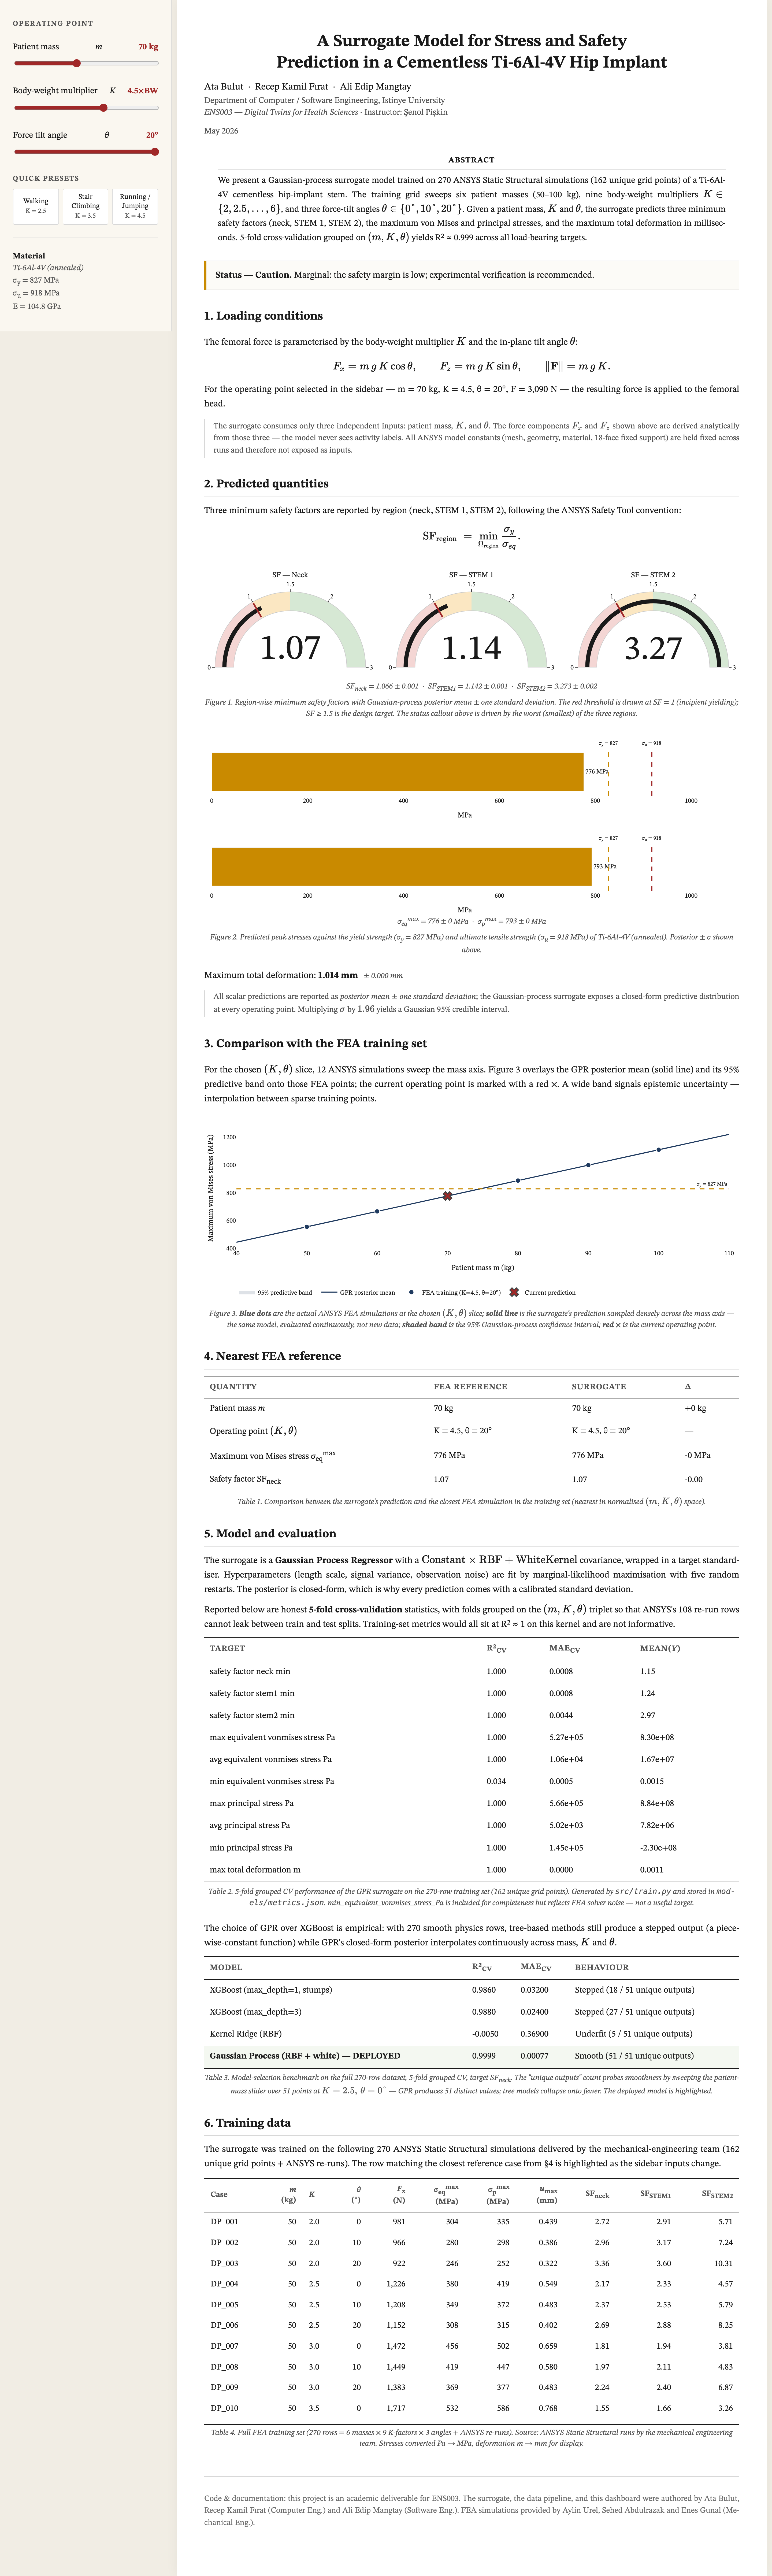
\includegraphics[width=0.78\textwidth]{../../screenshots/desktop_1440__tilted_70kg_K4.5_20deg.png}
  \end{center}
  \vspace{-0.4cm}
  \footnotesize
  \(m{=}70\unit{kg}\), \(K{=}4.5\), \(\theta{=}20°\) operating point.
  3 SF gauge'tan SF\(_{\text{neck}}{=}1.07\) (Caution), SF\(_{\text{stem2}}{=}3.27\)
  (Safe). Sağ kolonda nearest FEA referansı: eğitim satırı birebir eşleşiyor.
\end{frame}

% ---------------------------------------------------------------------------
\begin{frame}{Polish detayları}
  \begin{itemize}
    \item \textbf{Cache disable:} \code{SEND\_FILE\_MAX\_AGE\_DEFAULT=0}
          \(\Rightarrow\) Her CSS/JS düzenlemesi normal refresh'te görünüyor
          (dev verimliliği)
    \item \textbf{Mobile sidebar:} \code{@media (max-width: 760px)} ile
          slide-in panel; hamburger toggle butonu
    \item \textbf{Posterior \(\pm\sigma\) annotations:} GPR'nin standart
          sapması her gauge ve stress bar yanında italik gri olarak gösteriliyor
    \item \textbf{Activity preset butonları:} Sadece \(K\) slider'ını set
          ediyor --- mass ve angle korunuyor, user'ın seçimleri yerinde kalıyor
    \item \textbf{Training table scroll + sticky thead:} 270 satır, 460px
          yükseklik, kaydırırken başlık sabit
  \end{itemize}
\end{frame}

% ---------------------------------------------------------------------------
\begin{frame}[fragile]{CLI + entegrasyon}
\begin{lstlisting}[language=bash, basicstyle=\ttfamily\small]
$ ./run.sh predict --mass 70 --k 2.5 --angle 0
{
  "safety_factor_neck_min": 1.553,
  "safety_factor_stem1_min": 1.662,
  "safety_factor_stem2_min": 5.711,
  "max_equivalent_vonmises_stress_Pa": 532000000.0,
  ...
}

$ ./run.sh predict --mass 80 --activity stair_climbing
# K=3.5 preset'e snap'ler, sonra predict
\end{lstlisting}

  \vspace{0.4cm}
  Hem dashboard hem CLI \alert{aynı} \code{predict()} fonksiyonunu kullanıyor.
  \code{preprocess.add\_features()} \(\Rightarrow\) tek doğruluk kaynağı.
\end{frame}

% ---------------------------------------------------------------------------
\begin{frame}{Deploy yolu (açık karar)}
  \textbf{Şu an:} \code{flask run} dev server, Python deps \(\sim 234\) MB

  \vspace{0.3cm}
  \textbf{Vercel/Netlify serverless:} 250 MB unzipped limit --- sınırda,
  cold start 3-5 sn

  \vspace{0.4cm}
  \textbf{Aday yollar:}
  \begin{enumerate}\small
    \item Hugging Face Spaces / Render / Railway (Flask olduğu gibi)
    \item Plotly client-side'a it (\(\sim 40\) MB tasarruf)
    \item \alert{Statik precompute:} \((m, K, \theta)\) grid'ini önceden
          örnekle, \(\sim 1\) MB gzip JSON, frontend trilinear interpolation
          \(\Rightarrow\) GitHub Pages, sıfır backend
    \item GPR'yi JS'e port et (\(\sim\) 100 satır), exact predictions
  \end{enumerate}

  \vspace{0.3cm}
  Bu sunumun ardından ekip kararına göre yapılacak.
\end{frame}

% ---------------------------------------------------------------------------
\begin{frame}{Sorular}
  \vfill
  \begin{center}
    \Large Teşekkürler.\\[0.4cm]
    \normalsize Sorular?
  \end{center}
  \vfill
  \scriptsize
  \begin{itemize}
    \item \file{src/app.py}, \file{src/predict.py}, \file{src/templates/}, \file{src/static/}
    \item \file{run.sh} (CLI wrapper)
    \item \file{scripts/capture\_screenshots.py} (dashboard görselleri)
    \item Sprint logu: \file{docs/PROJECT\_NOTES.md} Sprint 4, 7
  \end{itemize}
\end{frame}

\end{document}
